
$\triangle ABC$ and $\triangle DBC$ are two isosceles triangles on the same base $BC$ and the vertices $A$ and $D$ are on the same side of $BC$. If $AD$ is extended to intersect $BC$ at $P$, show that \\
a) $\triangle ABD$ $\cong$ $\triangle ACD$ \\
b) $\triangle ABP$ $\cong$ $\triangle ACP$ \\
c) $AP$ bisects $\angle A$ as well as $\angle D$\\
d) $AP$ is the parpendicular bisector of $BC$

\begin{figure}[!ht]
\centering
\resizebox{\columnwidth}{!}{%
%
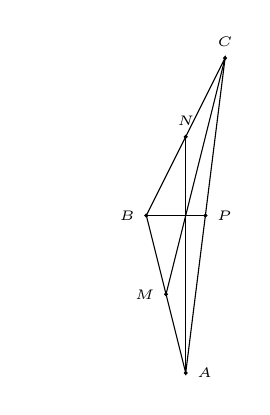
\begin{tikzpicture}
%[scale=0.5,>=stealth,point/.style={draw,circle,fill = green,inner sep=0.1pt},]
[scale=0.5,>=stealth, point/.style={draw,circle,fill = black,inner sep=0.1pt}]


%%
%%%Triangle sides
\def\a{4.12}
\def\b{4.47}
%\def\c{sqrt(\a^2+\c^2)}
\def\c{8.06}
%%
%%
%%
%%%Labeling points
%\node (A) at (0,\b)[point,label=above right:$A$] {};
%\node (B) at (\a, 0)[point,label=below left:$B$] {};
%\node (C) at (0, 0)[point,label=below right:$C$] {};
%\node (M) at (\a*0.5,\b*0.5)[point,label=above:$M$] {};
%\node (D) at (\a,\b)[point,label=above right:$D$] {};
%%
%%
%%%Drawing triangle ABC
%\draw (A) -- node[below] {$\textrm{}$} (B) -- node[left] {$\textrm{a}$} (C) -- node[above,xshift=5mm] {$\textrm{b}$} (A);
%%
%%%Joining CD
%\draw (C)--(D);
%%%Joining BD
%\draw (B)--(D);
%%
%%%Drawing and marking angles
%%\tkzMarkAngle[fill=orange!40,size=0.5cm,mark=](A,M,C)
%%\tkzMarkAngle[fill=orange!40,size=0.5cm,mark=](B,M,D)
%%\tkzMarkAngle[fill=green!40,size=0.5cm,mark=](A,B,C)
%%\tkzMarkRightAngle[fill=blue!20,size=.2](A,C,B)
%%\tkzMarkRightAngle[fill=blue!20,size=.2](D,B,C)
%%\tkzLabelAngle[pos=0.65](A,M,C){$\theta$}
%%\tkzLabelAngle[pos=0.65](B,M,D){$\theta$}
%%\tkzLabelAngle[pos=0.65](A,B,C){$\alpha$}
%%


% the coordinates of the vertices
\coordinate (A) at (4,-6);
\coordinate (B) at (3,-2);
\coordinate (C) at (5,2);


\coordinate (M) at (3.5,-4);
\coordinate (N) at (4,0);
\coordinate (P) at (4.5,-2);

% the axis
\draw[thin,scale=0,-] (-1,0) -- (5.5,0);
\draw[thin,scale=0,-] (0,-2.5) -- (0,2.5);

% the edges of the triangle
\draw (A) -- (B) -- (C) -- cycle;
\draw[-] (B) -- (P) ;
\draw[-] (A) -- (N) ;
\draw[-] (C) -- (M) ;

% labelling the vertices
%\node (A) at (4,-6)[point,label=above right:$A$] {};
\node[point,label={right:\tiny $A$}] at (A) {};
\node[point,label={left:\tiny $B$}] at (B) {};
\node[point,label={above:\tiny $C$}] at (C) {};
\node (M) at (3.5,-4)[point,label=left:\tiny $M$]{};
\node (N) at (4,0)[point,label=above:\tiny $N$] {};
\node (P) at (4.5,-2)[point,label=right:\tiny $P$] {};

% the arcs for the angles
%\begin{scope}[black]
%\draw[->]
%  (1,0) +(0:0.5cm) arc [radius=1cm,start angle=0,end angle=41] node[midway,right] {$\alpha$};
%\draw[->]
%  (0.5,0) +(0:0.25cm) arc [radius=0.75cm,start angle=0,end angle=122] node[midway,above] {$\beta$};
%\end{scope}
%
\end{tikzpicture}
%



%\begin{tikzpicture}[scale=.5]
%  \tkzDefPoint(4,-6){A} \tkzDefPoint(3,-2){B}
%  %\tkzDrawCircle[R,dashed](A,7 cm) \tkzDrawCircle[R,dashed](B,13 cm)
%  \tkzInterCC[R](A,4.12 cm)(B,4.47 cm) \tkzGetPoints{C}{D}
%  \tkzDrawPolygon(A,B,C)
%  \tkzCompasss(A,C B,C)
%  \tkzLabelSegment[below](A,B){$4.12$ cm}
%  \tkzLabelSegment[above left](A,C){$4.47$ cm}
%  \tkzLabelSegment[above right](B,C){$8.06$ cm}
%  \tkzDrawPoints[color=red](C)
%  \tkzDrawPoints[color=blue](A,B)
%\end{tikzpicture}
}
\caption{Iso-sceles Triangles by Latex-Tikz}
\label{eq:solutions/1/33/fig:iso_scelen}	
\end{figure}

The above problem statement is depicted in the figure \ref{eq:solutions/1/33/fig:iso_scelen} where the vertices are: A, B and C for $\triangle ABC$ and D, B and C for $\triangle DBC$. For $\triangle ABC$ the sides AB, BC and CA are represented by the vectors $\vec{A-B}$ , $\vec{B-C}$ and $\vec{C-A}$ and for $\triangle DBC$ the sides DB, BC and CD are represented by $\vec{D-B}$ , $\vec{B-C}$ and $\vec{C-D}$.

From the problem statement we get that:
\begin{equation}
\begin{aligned}
\norm{\vec{A}-\vec{B}} = \norm{\vec{A}-\vec{C}}
%\implies \norm{\vec{AB}} = \norm{\vec{AC}}
\end{aligned}
\end{equation}
\label{eq:solutions/1/33/cond1}
\begin{align}
\norm{\vec{D}-\vec{B}} = \norm{\vec{D}-\vec{C}}
%\implies \norm{\vec{DB}} = \norm{\vec{DC}}
\end{align}
\label{eq:solutions/1/33/cond2}
\begin{align}
\vec{P-C} = K_2 (\vec{B-C})\\
\vec{P-B} = K_1 (\vec{B-C})
\end{align}
\begin{multline}
\norm{\vec{A-B}} = \norm{\vec{A}-\vec{C}}\\
\implies \norm{\vec{A-B}}^2 = \norm{\vec{A-C}}^2\\
\implies \norm{{(\vec{A-P}) + (\vec{P-B})}}^2 = \norm{{(\vec{A-P}) + (\vec{P-C})}}^2\\
\implies \norm{\vec{A-P}}^2 + \norm{\vec{P-B}}^2 + 2(\vec{A-P})^T (\vec{P-B})=\\
\norm{\vec{A-P}}^2 + \norm{\vec{P-C}}^2 + 2(\vec{A-P})^T (\vec{P-C})\\
\implies \norm{\vec{P-B}}^2 + 2(\vec{A-P})^T (\vec{P-B})=\\
\norm{\vec{P-C}}^2 + 2(\vec{A-P})^T (\vec{P-C})\\
\implies \norm{\vec{P-B}}^2 -\norm{\vec{P-C}}^2\\
 + 2(\vec{A-P})^T ((\vec{P-B})-(\vec{P-C})) =0\\
\implies ((\vec{P-B})+(\vec{P-C}))^T ((\vec{P-B})-(\vec{P-C}))\\
+ 2(\vec{A-P})^T ((\vec{P-B})-(\vec{P-C})) =0\\
\implies (\vec{B}+\vec{C}-2\vec{P})^T (\vec{B-C})\\
+2(\vec{A-P})^T (\vec{P}-\vec{B}-\vec{P}+\vec{C}) =0\\
\implies (\vec{B}+\vec{C}-2\vec{P})^T (\vec{B-C})+2(\vec{A-P})^T (\vec{B-C}) =0\\
\implies ((\vec{B}+\vec{C}-2\vec{P})^T - 2(\vec{A-P})^T)(\vec{B-C})=0\\
\implies ((\vec{B}+\vec{C}-2\vec{P})-(\vec{2A-2P}))^T (\vec{B-C})=0\\
\implies (\vec{B+C-2A})^T (\vec{B-C})=0\\
\implies (\vec{B-C})^T (\vec{B+C-2A})=0\\
\label{eq:solutions/1/33/cond3}
\end{multline}
Now, from \ref{eq:solutions/1/33/cond3}
\begin{multline}
(\vec{B-C})^T \brak{\vec{\brak{\frac{B+C}{2}}-A}}=0\\
\implies \brak{\vec{\brak{\frac{B+C}{2}}-A}} \perp (\vec{B-C})
\end{multline}
So, we can conclude that $\vec{A-P}$ bisects $\vec{B-C}$ perpendicularly.
Similarly, 
\begin{multline}
\norm{\vec{D-B}} = \norm{\vec{D-C}}\\
\implies \norm{\vec{D-B}}^2 = \norm{\vec{D-C}}^2\\
\implies \norm{{(\vec{D-P}) + (\vec{P-B})}}^2 = \norm{{(\vec{D-P}) + (\vec{P-C})}}^2\\
\implies \norm{\vec{D-P}}^2 + \norm{\vec{P-B}}^2 + 2(\vec{D-P})^T (\vec{P-B})=\\
\norm{\vec{D-P}}^2 + \norm{\vec{P-C}}^2 + 2(\vec{D-P})^T (\vec{P-C})\\
\implies \norm{\vec{P-B}}^2 + 2(\vec{D-P})^T (\vec{P-B})=\\
\norm{\vec{P-C}}^2 + 2(\vec{D-P})^T (\vec{P-C})\\
\implies \norm{\vec{P-B}}^2 -\norm{\vec{P-C}}^2\\
 + 2(\vec{D-P})^T ((\vec{P-B})-(\vec{P-C})) =0\\
\implies ((\vec{P-B})+(\vec{P-C}))^T ((\vec{P-B})-(\vec{P-C}))\\
+ 2(\vec{D-P})^T ((\vec{P-B})-(\vec{P-C})) =0\\
\implies (\vec{B}+\vec{C}-2\vec{P})^T (\vec{B-C})\\
+2(\vec{D-P})^T (\vec{P}-\vec{B}-\vec{P}+\vec{C}) =0\\
\implies (\vec{B}+\vec{C}-2\vec{P})^T (\vec{B-C})+2(\vec{D-P})^T (\vec{B-C}) =0\\
\implies ((\vec{B}+\vec{C}-2\vec{P})^T - 2(\vec{D-P})^T) (\vec{B-C})=0\\
\implies ((\vec{B}+\vec{C}-2\vec{P})-(\vec{2D-2P}))^T (\vec{B-C})=0\\
\implies (\vec{B+C-2D})^T (\vec{B-C})=0\\
\implies (\vec{B-C})^T (\vec{B+C-2D})=0\\
\label{eq:solutions/1/33/cond4}
\end{multline}
Similarly, \ref{eq:solutions/1/33/cond4} dividing by 2, we get:
\begin{multline}
(\vec{B-C})^T \brak{\vec{\brak{\frac{B+C}{2}}-D}}=0\\
\implies \brak{\vec{\brak{\frac{B+C}{2}}-D}} \perp (\vec{B-C})
\end{multline}
So, we can conclude that $\vec{D-P}$ bisects $\vec{B-C}$ perpendicularly.
\renewcommand{\theequation}{\theenumi}
%\begin{enumerate}[label=\thesection.\arabic*.,ref=\thesection.\theenumi]
%\numberwithin{equation}{enumi}
%\item Verification of the above problem using python code.\\
%%\solution The  following Python code generates Fig. \ref{eq:solutions/1/33/fig:point_distance}
%%\begin{lstlisting}
%%codes/det_check.py
%%\end{lstlisting}
%
%\end{enumerate}




